\documentclass{cmn}

\newcommand\vsep{7mm}
\newcommand\textwidthfirst{50mm}
\newcommand\textwidthsecond{76mm}

\begin{document}
  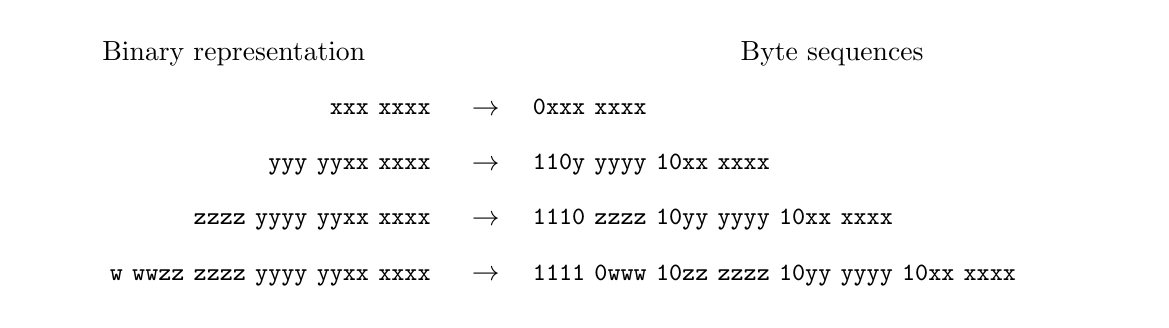
\begin{tikzpicture}
    \node[text width=\textwidthfirst,align=center] at (0,0) {Binary representation\strut};
    \node[text width=\textwidthfirst,align=right] at (0,-1*\vsep) {\small\texttt{xxx xxxx}\strut};
    \node[text width=\textwidthfirst,align=right] at (0,-2*\vsep) {\small\texttt{yyy yyxx xxxx}\strut};
    \node[text width=\textwidthfirst,align=right] at (0,-3*\vsep) {\small\texttt{zzzz yyyy yyxx xxxx}\strut};
    \node[text width=\textwidthfirst,align=right] at (0,-4*\vsep) {\small\texttt{w wwzz zzzz yyyy yyxx xxxx}\strut};

    \node at (32mm,-1*\vsep) {$\rightarrow$\strut};
    \node at (32mm,-2*\vsep) {$\rightarrow$\strut};
    \node at (32mm,-3*\vsep) {$\rightarrow$\strut};
    \node at (32mm,-4*\vsep) {$\rightarrow$\strut};

    \node[text width=\textwidthsecond,align=center] at (76mm,0) {Byte sequences};
    \node[text width=\textwidthsecond,align=left] at (76mm,-1*\vsep) {\small\texttt{0xxx xxxx}\strut};
    \node[text width=\textwidthsecond,align=left] at (76mm,-2*\vsep) {\small\texttt{110y yyyy 10xx xxxx}\strut};
    \node[text width=\textwidthsecond,align=left] at (76mm,-3*\vsep) {\small\texttt{1110 zzzz 10yy yyyy 10xx xxxx}\strut};
    \node[text width=\textwidthsecond,align=left] at (76mm,-4*\vsep) {\small\texttt{1111 0www 10zz zzzz 10yy yyyy 10xx xxxx}\strut};

  \end{tikzpicture}
\end{document}
